%Original creator: Tim Rentenaar
%Format inspired by FUZE TEAM's INFOMDWR midterm cheat sheet
%When editing and/or sharing this file please credit the original creator

\documentclass[a4paper,7pt,landscape]{extarticle}
\usepackage{extsizes}
\usepackage[a4paper,margin=0.1cm,nohead,foot=0.5cm]{geometry}
\usepackage{graphicx} % Required for inserting images
\usepackage{multicol} % for multicolumn layout
\usepackage[many]{tcolorbox}
\usepackage{amsmath, amssymb}

\newcommand{\indep}{\perp \!\!\! \perp} % independence symbol
\newcommand{\nindep}{\not\!\perp\!\!\!\perp} % not independence symbol
\DeclareMathOperator*{\E}{\mathbb{E}} % Expectation symbol

\setlength{\columnsep}{0.1cm}
\pagenumbering{gobble}

%boxes source: https://www.overleaf.com/latex/examples/simple-stylish-box-design/stzmmcshxdng
\tcbset{
    breakable,
    sharp corners,
    colback = white,
    %before skip = 0.1cm,    % add extra space before the box
    %after skip = 0.1cm      % add extra space after the box
}                           % setting global options for tcolorbox

\newtcolorbox{boxA}{
    %fontupper = \bf,
    boxrule = 1.5pt,
    colframe = black % frame color
}

\begin{document}

\begin{multicols}{3} %no of columns
\fontsize{6.2pt}{1pt}\selectfont

INFOMDCSBS Cheat Sheet - Created by Tim Rentenaar

\begin{boxA}
\underline{\textbf{Lecture 1: Introduction to Causal Inference}}\\
\textbf{Randomized Controlled Trial (RCT):} A sample get split randomly into two groups: group with the controlled condition, and group with the experimental condition. Because of this split, the groups are seen as equal. If we find a difference, it must be caused by the experiment.\\
\textbf{Marginal Distribution:} The probability distribution of one variable where other variables are not taken into account\\
\textbf{Joint Distribution:} The probability distribution of two or more variables. It describes the simultaneous occurrence of values for each variable in a given set.\\
\textbf{Conditional Distribution:} The probability distribution of one variable in a set of variables where other variable(s) are set to a certain value\\
\textbf{Confounder:} A common cause of the two variables we are interested in\\
\textbf{Conditioning:} Remove the effect of the confounding variable by selecting a group within the confounding variable\\
\textbf{Conditioning Methods:} Select particular group within confounding variable; Create groups based on confounding variable (i.e. strata); Match individuals within the confounding variable; Use multiple regression analysis with the confounding variable as a covariate;\\
\textbf{Mediator:} A variable is a mediator when it's on the causal path from one variable to the other\\
\textbf{Causal statements:} Should be based on: The outcome of an action, applied to a unit at a particular point in time relative to the outcome of another action.\\
\textbf{Potential outcomes:} The potential outcome when given treatment (X=1): $Y^{x=1}$. The potential outcome when not given treatment (X=0): $Y^{X=0}$.\\
\textbf{Fact vs Counterfact:} Only one potential outcome can be observed. The potential outcome we do observe is fact. The potential outcome we do not observe is counterfact.\\
\textbf{Individual Causal Effect (ICE):} The difference in potential outcomes of individuals: $ICE_i = Y_i^1-Y_i^0$\\
\textbf{Average Causal Effect (ACE):} As we cannot observe both potential outcomes, we typically focus on the average causal effect instead: $ACE = \E [Y_i^1-Y_i^0] = \E [Y_i^1]- \E [Y_i^0]$\\
\textbf{Exchangeability Assumption:} Treatment is independent of potential outcomes: $Y_i^1, Y_i^0 \indep X_i$. This is also known as unconfoundedness or ignorability.\\
\textbf{Conditional Exchangeability:} $Y_i^1, Y_i^0 \indep X_i | Z_i$; Within a certain level of Z, the assignment is random. This is also known as no unobserved confounding.\\
\textbf{Positivity Assumption:} $0 < Pr(X = 1|Z)$ and $0 < Pr(X = 0|Z)$; There must be treated and untreated participants at every combination of values of Z in the population under study.\\
\textbf{Consistency Assumption:} $Y_i=Y_i^x$ for $X_i=x_i$; The observed outcome $Y_i$ equals the potential outcome that is associated with setting treatment to the level that was observed.\\
\textbf{Strong ignorability:} Positivity and Exchangability combined.\\
\textbf{Phase 1: Formulation:} What is the exact causal question? (population, timing etc.)\\
\textbf{Phase 2: Identification:} Given an infinitely large sample, can you determine the causal effect?\\
\textbf{Phase 3: Estimation:} Based on the identification assumptions, and additional assumptions, obtain an estimate\\
\textbf{Phase 4: Sensitivity Analysis:} How badly should assumptions be violated before the conclusions would change? (not in this course)
    
\end{boxA}

\begin{boxA}
\underline{\textbf{Lecture 2: Rubin Causal Model}}\\
\textbf{Stable Unit Treatment Value Assumption (SUTVA):} The potential outcomes for any unit do not vary with the treatments assigned to other units (i.e., no interference); For each unit, there are not different versions of each treatment level that lead to different potential outcomes. Note these issues are also captured by the consistency assumption.\\
\textbf{Estimand:} A quantity that is to be estimated in a statistical analysis.\\
\textbf{Estimator:} The method used to obtain an approximation of the estimand.\\
\textbf{Estimate:} The specific value obtained from a given method and dataset.\\
\textbf{ACE0:} Average Causal Effect for the untreated\\
\textbf{ACE1:} Average Causal Effect for the treated\\
\textbf{Standardized Mean Difference (SMD):} \\$\Delta Z = \frac{(\overline{Z} | X = 1)-(\overline{Z} | X = 0)}{\sqrt{((S^2 | X = 1)+(S^2 | X = 0)) / 2}}$ ; Where $\overline{Z}|X=x$ is the sample mean in condition $X=x$, and $S^2|X=x$ is the sample variance in group X=x.\\
\textbf{4 main strategies when controling for covariates:}\\
\textbf{No confounders included:} Naive approach (Method 1)\\
\textbf{Model the relation between confounders (Z) and outcome (Y):} Goal is to account for confounding through including confounders (Methods 2 and 3)\\
\textbf{Model the relation between confounders (Z) and treatment (X):} Goal is to change the data to what would have been obtained in an RCT (Methods 4, 5, and 6)\\
\textbf{Model the relation between confounders (Z) and treatment (X) AND outcome (Y):} Goal is to be correct in at least one of these parts (Methods 7, 8 , and 9)\\
\textbf{1. Simple difference in means / Prima Facie Effect:} $PFE = \E [Y_i^1|X_i=1]- \E [Y_i^0|X_i=0]$; This mean difference can be estimated using a t-test (or a regression analysis with a dummy as predictor).\\
\textbf{2a. ANCOVA (regression without interactions):} $Y_i = \alpha+\theta X_i+ \beta_1 Z_{i1}+…+\beta_p Z_{ip}+e_i$; We interpret $\theta$ as the causal effect of X.\\
\textbf{2b. Regression analysis (with interactions):} $Y_i = \alpha+\theta X_i + \beta_1 Z_{i1}+…+\beta_p Z_{ip}+ \gamma_1 X_i \times Z_{i1}+…+ \gamma_p X_i \times Z_{ip}+e_i$; $\beta$ are the slopes in the control group ($X_i=0$), $\gamma$'s are the differences in slopes between the treatment group ($X_i=1$) and the control group ($X_i=0$).\\
\textbf{3. Regression estimation:} Potential outcomes can be estimated by the regression. $\hat{ACE} = \frac{1}{N} \sum_{i=1}^N (\hat{Y}_i^1 - \hat{Y}_i^0)$\\
\textbf{Propensity scores:} Probability of being treated: $\pi_i = P[X_i = 1 | Z_i] = \frac{exp(Z_i' \phi)}{1 + exp(Z_i' \phi)}$\\
\textbf{4. Matching:} Matching implies you create pairs that consist of a treated and a non-treated person, who have identical propensity scores. Balancing property: $P(Z|\pi = c,X = 1) = P(Z|\pi = c,X = 0)$. If the propensity model is correct, then comparing treated and untreated individuals with the same $\pi$ is a way of mimicking an RCT. Note that this gives us ACE1 or ACE0 (depending on which group is the smallest), rather than ACE.\\
\textbf{5. Inverse probability weighting:} The probability of received treatment is: $\pi_i$ for those who were treated $(X_i = 1)$, and $1 - \pi_i$ for those who were NOT treated $(X_i = 0)$. To account for the representation imbalance, we create a pseudo-population where each case is weighted by the inverse probability of received treatment:  $\frac{1}{\hat{\pi}_i}$ for $X_i = 1$, and $\frac{1}{1-\hat{\pi}_i}$ for $X_i = 0$.\\
\textbf{IPW estimate of ACE:} $\hat{ACE} = \frac{\sum_i X_i Y_i / \hat{\pi}_i}{\sum_i X_i / \hat{\pi}_i} - \frac{\sum_i (1-X_i) Y_i / (1 - \hat{\pi}_i)}{\sum_i (1-X_i) / (1- \hat{\pi}_i)}$\\
\textbf{6. Stratification:} Propensity scores can be used to create strata. ACE of each stratum can be estimated. The stratum specific ACEs can be combined into an overall ACE.\\
 \textbf{Doubly-Robust:} Combined modeling strategies. As long as one of the two models is correctly specified, the other can be misspecified without harm.\\
\textbf{7. Weighted residual bias corrections:} This approach is related to method 3 and 5. Residuals are estimated using the estimated potential outcomes: $\hat{\epsilon}_i^1 = Y_i^1 - \hat{Y}_i^1$ and $\hat{\epsilon}_i^0 = Y_i^0 - \hat{Y}_i^0$. $ACE = \frac{1}{N} \sum_{i=1}^N (\hat{Y}_i^1 - \hat{Y}_i^0) + \frac{\sum_i X_i \hat{\epsilon}_i^1 / \hat{\pi}_i}{\sum_i X_i / \hat{\pi}_i} - \frac{\sum_i (1-X_i) \hat{\epsilon}_i^0 / (1 - \hat{\pi}_i)}{\sum_i (1-X_i) / (1- \hat{\pi}_i)}$\\
\textbf{8. Weighted regression estimation:} This method is similar to method 3, but the big difference is that while estimating $\hat{\beta}_0$ and $\hat{\beta}_1$, the inverse probability weights $\frac{1}{\pi_i}$ and $\frac{1}{1-\pi_i}$ are used for correction.\\
\textbf{9. Regression with propensity-related covariates:} Make dummy variables based on the propensity score (say 10 dummies); this is similar to making the strata for Method 6. Next, include these dummies (but one) in a regression model (as Method 3): estimate $\hat{\beta}_1$ for the treated, and $\hat{\beta}_0$ for the non-treated; based on these estimated regression coefficients, estimate the potential outcomes $\hat{Y}_i^1$ i and $\hat{Y}_i^0$ for everyone.
    
\end{boxA}

\begin{boxA}
\underline{\textbf{Lecture 3: Directed Acyclic Graphs (DAGs)}}\\
\textbf{Causal Graphs:} Represents our knowledge and ideas about The Truth. Consists of: nodes: these are variables; edges: these are connections between nodes. when they are one-headed arrows, we call them directed edges.\\
\textbf{Three basic Causal Graph structures:} Fork; Chain; Inverted Fork.\\
\textbf{Fork:} $X \leftarrow Z \rightarrow Y$. $X \nindep Y$; $X \indep Y | Z$. Z is a confounder.\\
\textbf{Chain:} $X \rightarrow Z \rightarrow Y$. $X \nindep Y$; $X \indep Y | Z$. Z is a mediator.\\
\textbf{Inverted Fork:} $X \rightarrow Z \leftarrow Y$. $X \indep Y$; $X \nindep Y | Z$. Z is a collider.\\
\textbf{Confounder bias:} A path with a confounder can be closed by conditioning on the confounder. Failing to close this path leads to confounder bias.\\
\textbf{Overcontrol bias:} To determine the total causal effect, we should NOT condition on the mediator. This would lead to overcontrol bias.\\
\textbf{Collider bias / Selection bias:} Conditioning on a collider opens a blocked path. This would lead to collider bias or selection bias.\\
\textbf{Direct causal path:} A path with one arrow from the exposure to the outcome.\\
\textbf{Indirect causal path:} A path leading from the exposure to the outcome with one or more mediators.\\
\textbf{Non-causal path:} A path that doesn't lead from the exposure to the outcome.\\
\textbf{Back-door path:} Any path connecting the exposure and the outcome, starting with an arrow pointing into the exposure.\\
\textbf{Open back-door path:} A back-door path that contributes to the association between the exposure and the outcome; it contains a common cause of the exposure and the outcome. It can be blocked by conditioning on the common cause, or any other variable along the path; these are referred to as (proxy) confounders.\\
\textbf{Closed back-door path:} A back-door path that does not contribute to the association between the exposure and the outcome; it contains a collider. It can be opened by conditioning on the collider.\\
\textbf{Family language}: $A \rightarrow B \rightarrow C$: A is the parent of the child B. A is the ancestor of the descendant C.\\
\textbf{Causal identification using a DAG: Step 1:} Determine all paths that connect the exposure and the outcome.\\
\end{boxA}

\begin{boxA}
\textbf{Causal identification using a DAG: Step 2:} Once we know all the paths, we can use Pearl’s back-door criterion, which consists of two conditions. Condition 1: Find a set of covariates Z, which closes all back-door paths. Condition 2: Check that none of the covariates in Z are descendants of the exposure.\\
\textbf{D-seperated:} When both conditions of Pearl's back-door criterion are met, we can say that conditional on Z, X and Y are d-separated.\\
\textbf{Major strength of back-door criterion:} The rules for the back-door criterion are mathematical; they can be performed by a computer algorithm.\\
\textbf{M-bias:} $X \leftarrow Z_1 \rightarrow W \leftarrow Z_2 \rightarrow Y$. Suppose $Z_1$ and $Z_2$ are unobserved, should we condition on $W$? $W$ is a collider; conditioning on it opens a back-door path through $Z_1$ and $Z_2$ leading to collider bias. This collider bias is also known as M-bias.\\
\textbf{Do-operator:} A surgical (hypothetical) intervention. Confounding: $P(Y|X) \neq P(Y|do(X))$. Where: do(X) is the surgical intervention; P(Y|X) is the conditional probability of the outcome given the treatment; P(Y|do(X)) is the intervention probability. Causal effect: $E[Y|do(X = 1)]-E[Y|do(X = 0)]$\\
\textbf{PO framework vs Pearl's framework:} Target trial: In the PO framework, the target trial is considered an important tool. For Pearl, this is an unnecessary limitation; Attributes: Related to this, when it is hard to imagine how to intervene on something (e.g., race, sex at birth, age), this cannot be conceived of as a cause in the PO framework, and it is referred to as an attribute. For Pearl, there is no need to make this distinction; Consistency: In the PO framework, the assumption of consistency is a key identification assumption. For Pearl, this follows automatically; Confounding: In the PO framework, confounding is defined in terms of potential outcomes. Pearl defines it directly in terms of the outcome (although also hypothetical).\\
\textbf{Pearl’s ladder of causation:} A hierarchy of problems: Rung 1: prediction: requires seeing. Rung 2: intervening: requires the do-operator and results in the ACE. Rung 3: counterfactual reasoning: requires the structural causal model (SCM) and provides the individual’s counterfactuals (and the ICE).\\
\textbf{Structural Causal Model components:} Exogenous variables U; Endogenous variables V; Functions that map U to V.\\
\textbf{Simpson's paradox:} Two variables are statistically dependent in the general population, and this relation is reversed or absent when looking at sub-populations.\\
\textbf{Berkson's paradox:} Two variables are statistically independent in the general population, but statistically dependent in a sub-population that was selected.\\
\textbf{Instrumental variable:} When we want to estimate the causal effect between X and Y but there is a confounder Z, the causal effect can be estimated with an instrument variable. Assumptions: 1 effects are linear; 2 instrument is correlated with treatment (can be tested); 3 instrument is not caused by hidden confounder; 4 instrument only affects outcome through treatment.\\
\textbf{Mendelian Randomization:} Mendelian randomization is used a lot in epidemiological research. It is based on using a genotype score (either a single nucleotide polymorphism (SNP) or a polygenic risk score (PRS)) as the instrumental variable. In principle, the genotype score should affect the outcome only through the exposure, but it may be possible to block other (indirect) paths.\\
\textbf{Front-door Criterion:} Pearl's example: does smoking cause lung cancer? How to estimate the causal effect when there might be an unmeasured gene that causes both the tendency to smoke and lung cancer? Answer: introduce a mediator between smoking and lung cancer: tar and: determine the effect of tar on lung cancer, conditional on smoking; determine the effect of Smoking on tar; combine to get the effect of smoking on lung cancer. Main issue: exposure should affect outcome only through the mediator; mediator should not be affected by confounder(s) only through exposure.
    
\end{boxA}

\begin{boxA}
\underline{\textbf{Lecture 4: Causal Discovery}}\\
\textbf{Global Markov Condition:} Every variable (node) is conditionally independent of its non-descendants, given its parents: $X \indep non-descendants(X) | parents(X)$.\\
\textbf{D-seperation rules:} Marginal (in)dependencies: Chains and Forks are open paths; Collider structures are blocked paths. Conditional (in)dependencies: Conditioning on Mediators and Confounders or their descendants block a path; Conditioning on Colliders or their descendants open a path.\\
\textbf{Causal discovery with DAGs:} Basic idea: 1 Find all marginal and conditional (in)dependence relations present in the data. 2 Draw the DAG(s) that match (only) those (in)dependencies, given the d-seperation rules. Relevant Assumptions: The causal system of interest can be captured in a DAG; No unobserved confounding (Sufficiency, conditional exchangeability); No conditioning on unobserved colliders (no selection bias); Faithfulness; Various statistical assumptions for evaluating statistical dependencies.\\
\textbf{Causal discovery with independence tests and DAGs - Step 1:} Draw undirected edges between variables you are sure have to be there, based on independence tests. Principle 1: Two variables A and B are directly connected in the DAG (either $A \rightarrow B$ OR $B \rightarrow A$) - if, and only if - they are dependent conditional on every possible subset of the other variables.\\
\textbf{Skeleton:} A structure of nodes and undirected edges.\\
\textbf{Moral Skeleton:} If the skeleton has two variables with a common child, an edge is added between the parent variables to create a moral skeleton.\\
\textbf{Causal discovery with independence tests and DAGs - Step 2:} Infer the direction of as many of the undirected edges as possible. Principle 2: If our skeleton contains a triplet X - Z - Y, where X and Y are not directly connected, we can orientate the arrows as $X \rightarrow Z \leftarrow Y$ - if and only if - X and Y are dependent conditional on every set of variables containing Z.\\
\textbf{Markov Equivalence:} Two DAGs are Markov Equivalent if they satisfy the same d-separation statements, that is, the same set of (conditional) (in)dependence relations.\\
\textbf{Complete Partially-Oriented Directed Acyclic Graph (CPDAG):} The Markov-Equivalance can be represented by a single CPDAG. Edges that could be pointed in either direction is represented as an undirected edge in the CPDAG.\\
\textbf{PC algorithm; FCI algorithm:} causal discovery algorithms that do a quicker search without having to test all (in)dependencies. Extensions exist that deal with violations of sufficiency. Still rely on faithfulness.\\
\textbf{Global Markov Condition:} If X and Y are d-separated by Z then $X \indep Y | Z$\\
\textbf{Faithfulness:} If $X \indep Y | Z$ then X and Y are d-separated by Z\\
\textbf{Violation of Faithfulness:} Violations of faithfulness can exist when paths perfectly cancel each other out. Example: $A = \epsilon_A$, $B = 0.5 A + \epsilon_B$, $C = -0.25A + 0.5B + \epsilon_C$: the effect of A on C is canceled out. On the population level faithfulness assumption is reasonable because paths never perfectly cancel out, but on the sample level faithfulness assumption is less reasonable.\\
\textbf{Causal discovery with independence tests and DAGs disadvantages:} Population (in)dependencies are estimated: uses sample data + statistical tests; CI testing easy if linear + Normal (partial correlation / regression) or discrete.\\
\textbf{Causal discovery with Invariant Causal Prediction (ICP):} Basic Idea: 1 There is some unknown causal graph, but we only care about learning the direct causes of one target variable Y; 2 We have data drawn from different environments; 3 We identify the direct causes of Y by looking for those conditional dependencies that are invariant (remain the same) across environments.\\
\textbf{ICP: Key assumptions:} Modularity and Localized Interventions:
Assuming it is possible to intervene on a variable without fundamentally changing how it relates to other variables. More specifically: Did not intervene on outcome variable Y (the effect); Interventions did not affect direct relations of interest; For the rest, less important what variables were intervened on or how.\\
\textbf{ICP disadvantages:} Sufficiency; Need different environments; Need knowledge that interventions are not directly on Y , or the direct relationships of
interest; Testing whether something is invariant may be hard; Can’t learn full graph.\\
\textbf{Adjacency matrix:} In the graphical modeling literature, the edges in a graph are represented by an adjacency matrix, typically denoted A. This is simply a matrix of 0’s and 1’s indicating which of the p variables share an edge (and hence the matrix will have a size of p×p). $A_{ij}=1$ indicates that there is an arrow from variable i to variable j, that is $X_i \rightarrow X_j$.

\end{boxA}

\begin{boxA}
\underline{\textbf{Lecture 5: Repeated Measures}}\\
\textbf{Lord's paradox:} ANCOVA and Change Score approaches for the analysis of change between two time-points can produce radically different results.\\
\textbf{Marginal model:} $Y_2 = \alpha_0 + \alpha_1 X + \delta$\\
\textbf{ANCOVA model:} $Y_2 = \beta_0 + \beta_1 X + \beta_2 Y_1 + e$. $ACE = \beta_1$\\
\textbf{Change score (or gain score) model:} $Y_2 - Y_1 = \gamma_0 + \gamma_1 X + \epsilon$. $ACE = \gamma_1$ or $ACE = (\mu_{2|1} - \mu_{1|1}) - (\mu_{2|0} - \mu_{1|0})$ or $ACE = (\mu_{2|1} - \mu_{2|0}) - (\mu_{1|1} - \mu_{1|0})$.\\
\textbf{What model to use with random assignment:} Pretest and treatment are unrelated: Marginal model; ANCOVA (more power).\\
\textbf{What model to use with assignment based on pretest:} Pretest is confounder: ANCOVA.\\
\textbf{What model to use for existing groups:} Pretest is a mediator: Marginal model for total effect; ANCOVA for direct effect only.\\
\textbf{Extending the DAGs to include the change score: pretest as confounder:} Need to block back-door paths. Use ANCOVA to get $X \rightarrow Y_2 \rightarrow G$.\\
\textbf{Extending the DAGs to include the change score: pretest as mediator:} Change score gives total effect; ANCOVA gives direct effect.\\
\textbf{Timing:} The DAGs show that the causal relation between treatment X and pre-test Y1 is critical; it is about whether X or Y1 came first (i.e., their temporal order). Covariates should come from the pre-exposure phase; then they cannot be affected by the treatment.\\
\textbf{ANCOVA and CSM under Five scenarios:}\\
\textbf{Scenario 1: No causal effect:} $\beta_1 = 0$, $\gamma_1 = 0$\\
\textbf{Scenario 2: CS model negative causal effect:} $\beta_1 = 0$, $\gamma_1 < 0$\\
\textbf{Scenario 3: ANCOVA model positive causal effect:} $\beta_1 > 0$, $\gamma_1 = 0$\\
\textbf{Scenario 4: Opposite conclusions regarding direction!:} $\beta_1 > 0$, $\gamma_1 < 0$\\
\textbf{Scenario 5: Some agreement:} $\beta_1 > 0$, $\gamma_1 > 0$\\
\textbf{Case when ACE of ANCOVA and CSM are identical:} Only when $\beta_2 = 1$ and/or $\mu_{1|1} = \mu_{1|0}$, are $\beta_1$ ($ACE_{ANCOVA}$) and $\gamma_1$ ($ACE_{CSM}$) identical.\\
\textbf{Pretest as a proxy of an unobserved confounder:} When there is an unmeasured confounder, $U$, that is a confounder of $X$, $Y_1$, and $Y_2$, $Y_1$ acts as a proxy of $U$ and controlling for $Y_1$ will partly remove bias due to $X \leftarrow U \rightarrow Y_2$. When we have linear relations (and the variance of U is equal to 1),  the two open back-door paths cancel each other out.\\    

\end{boxA}

\begin{boxA}
\underline{\textbf{Lecture 6: Joint Treatment Effects}}\\
\textbf{Longitudinal Process:} Exposure $X_t$, Covariates $L_t$, and Outcome $Y_t$, can take on varying values over time. Unvarying covariates $C$, stay the same over time and affect the process the same at each time point. Each $X_t$, $Y_t$, $L_t$ points into each $X_{t+1}$, $Y_{t+1}$, $L_{t+1}$.\\
\textbf{Point treatment:} All paths that lead from one exposure to the final outcome. Example: all paths $X_1 \rightarrow Y_4$ or $X_3 \rightarrow Y_4$.\\
\textbf{Joint Effect:} The effect of each exposure on the outcome not through subsequent exposure. “Joint” refers to “interventions” at multiple time points combined.\\
\textbf{Exposure regimes (static):} Predetermined rules that determine the value of a time-varying exposure for all time points jointly. For example: $\{X_1 = 2, X_2 = 1, X_3 = 0\}$ shortly represented as $\{2, 1, 0\}$\\
\textbf{Joint effect (in terms of regimes):} A contrast of outcomes that follow from two different exposure regimes. For example, for binary exposure, the always-exposed versus never-exposed effect can be represented as $Y^{\{1, 1, 1\}}$ versus $Y^{\{0, 0, 0\}}$\\
\textbf{Controlled Direct Effects (CDE):} Joint effects are a collection of controlled direct effects. A CDE is the effect of $X_t$ on $Y_T$,
unmediated by future exposure, $X_{t+1}$, $X_{t+2}$, etc\\
\textbf{Research question:} Must specify: target population ($ACE$, $ACE_0$, $ACE_1$?); exposure contrast (which regimes are compared and why?); outcome (how is it measured? when is it measured (time-lag)?).\\
\textbf{Causal estimand:} $ACE = \E [Y_T^{\overline{1}_{T-1}}] - \E [Y_T^{\overline{0}_{T-1}}]$. Exposure history up to $t$ is denoted as $\overline{X}_t$.\\
\textbf{Marginal Structural Model (MSM), general:} Maps a marginal expectation of potential outcomes, to treatments and parameters of interest. "Marginal" because we compare potential outcomes under two treatment regimes. "Structural" because it is a model for a specific aspect of the distribution of potential outcomes. From an MSM, we can compute what the expected potential outcome under a given treatment (regime). Then, we can compare different expected potential outcomes.\\
\textbf{MSM1:} $\E [Y^{\{x\}}] = \beta_0 + \beta_1 x$, where $x$ can only be $x = 0$ (representing $\overline{0}_T$) or $x = 1$ (representing $\overline{1}_T$). Is saturated (has as many variables as possible regimes)\\
\textbf{MSM2:} $\E [Y^{\{x_1,...,x_{T-1}\}}] = \psi_0 + \psi_1 x_1 + ... + \psi_{T-1} x_{T-1}$, possible for all exposure regimes. Is not saturated.\\
\textbf{MSM3:} $\E [Y^{\{x_1,x_2,x_3,...\}}] = \psi_0 + \psi_1 x_1 + \psi_2 x_2 + \psi_3 x_3 + \psi_4 x_1 x_2 + \psi_5 x_1 x_3 + \psi_6 x_2 x_3 + \psi x_1 x_2 x_3 + ...$, possible for al exposure regimes. Is saturated (but becomes impractical for more time points, and continuous exposures).\\
\textbf{Sequential conditional exchangeability:} $Y_T^{\overline{x}_t} \indep X_t | \overline{L}_{t}, \overline{A}_{t-1}$. In words: Conditional on treatment history up to time $t - 1$, and covariate history up to $t$, the received treatment at time $t$ is independent from the potential outcome.\\
\textbf{Sequential positivity:} $Pr[X_t | \overline{L}_t, \overline{A}_{t-1}] > 0$. In words: At each time point and across all values of the covariates in the data, there is a non-zero probability for individuals to be in either treatment condition.\\
\textbf{Sequential consistency:} For static regimes: If $\overline{X}_t = \overline{x}_t$ for a given individual, then $Y^{\overline{x}_t} = Y$ for that individual. If the treatment interventions at a particular time ($X_t = 1$ and $X_t = 0$) are well-defined for all treatment-times, then all regimes involving $X_t$ are also well-defined.\\
\textbf{Exposure-confounder feedback:} A specific situation in the context joint effects, where there exists a time-varying confounder $L_t$ that is independently associated with the outcome (directly, or by unmeasured common cause), predicts subsequent treatment $X_{t+1}$, and is affected by earlier treatment $X_{t-1}$.\\
\textbf{Inverse probability weighted estimation of marginal structural models (IPW-MSM):} Step by step: 1. Decide on covariates for which to balance (based on Phases I and II of causal research process); 2. (Examine the initial imbalance on each covariate, at each time point.); 3. Estimate a distance measure (here, the propensity score); 4. Condition on distance measure (here, weighting, rather than matching or sub-classification); 5 Assess imbalance in the reweighted sample with regards to relevant covariates; 6. Estimate treatment effect in the reweighted sample.\\
\textbf{Equation for each weight:} Final weight: $W_i = \prod_{t=1}^T W_{it}$, Weight at timepoint $t$: $W_{it} = X_{it} \frac{1}{Pr[X_{it} = 1 | \overline{L}_{it}, \overline{A}_{i,t-1}]}+(1-X_{it}) \frac{1}{1 - Pr[X_{it} = 1 | \overline{L}_{it}, \overline{A}_{i,t-1}]}$\\
\textbf{Stabilized weights:} $SW_{it} = X_{it} \frac{Pr[X_{it} = 1 | \overline{A}_{i,t-1}]}{Pr[X_{it} = 1 | \overline{L}_{it}, \overline{A}_{i,t-1}]}+(1-X_{it}) \frac{Pr[X_{it} = 1 | \overline{A}_{i,t-1}]}{1 - Pr[X_{it} = 1 | \overline{L}_{it}, \overline{A}_{i,t-1}]}$\\
\textbf{Estimate treatment effect in the reweighted sample:} Regress the outcome on the treatments in the balanced sample and calculate $ACE/ACE_0/ACE_1$.\\
\textbf{Advantages of IPW-MSM:} Researchers perceive this method as relatively simple; IPW procedures seperate confounding control and effect estimation; Balance of sample can be checked empirically; Many R packages exist for propensity score-based methods.\\
\textbf{IPW disadvantages:} Default IPW estimators are inefficient; Susceptible to bias when some confounders are strongly predictive of exposure, or when propensity score model is misspecified; Continuous exposure are, in principle, possible, but more complex to analyze using IPWs; Cannot accommodate effect modification by time-varying covariates.

\end{boxA}

\begin{boxA}
\underline{\textbf{Lecture 7: Unobserved Heterogeneity}}\\
\textbf{Cross-lagged panel research:} 2 or more waves of data; 2 or more variables. Does X affect Y, does Y affect X, which effect is larger (causally dominant)?\\
\textbf{Estimating the CLPM:} We can run: a seperate regression model for each outcome; Use structural equation modelling (SEM) to estimate it all at once.\\
\textbf{SEM and causality:} SEM are based on: strong causal assumptions: setting parameters to a particular value (e.g. 0). Tested with overall model fit; Weak causal assumptions: estimating parameters freely. Tested with parameter-specific test.\\
\textbf{Population heterogeneity:} Dynamic causal perspective: “victimization (offending) changes individuals in ways that alter their subsequent risk of offending (victimization)”; Population heterogeneity perspective: “victimization and offending are spuriously related, due to their common correlations with one or more underlying time-stable variable” e.g., personality traits, family or neighborhood factors.\\
\textbf{Retest correlation:} Correlation between 2 measurements of the same variable obtained from the same people on separate occasions. Two extreme cases: Retest correlation of 1: Perfect stability (only trait); Retest correlation of 0: No stability at all (only state). In general, retest correlations are larger when the interval between repeated measures is shorter.\\
\textbf{Trait-like and state-like sources of variance:} The correlation between the stable, trait-like components: trait correlation; The correlation between the temporal, state-like components: state correlation; The degree to which each variable consists of trait-like versus state-like components: intraclass correlations.\\
\textbf{Generalization slip (ecological fallacy):} When the characteristics of a group are attributed to an individual. (e.g. a group can have a negative correlation, but on an individual level it can be positive (words per minute / percentage of typos example))\\
\textbf{Random Intercept Cross-Lagged Panel Model (RI-CLPM):} Accounts for: Trait-like stability with the between part: this captures the unobserved heterogeneity; Moment-to-moment stability with the within part: this is where the dynamic relations are modeled.\\
\textbf{Intensive Longitudinal Data:} Many repeated measures. (e.g. daily diary, experience sampling method, ecological momentary assessment, real-time data capture, event-based measurements, observational measurements)\\
\textbf{Multilevel modeling:} Study relations in nested data. Within-person level: $y_{it} = \alpha_i + \beta_i x_{it} + e_{it}$; Between-person level: Random intercept: $\alpha_i = \gamma_{00} + u_{0i}$, Random slope: $\beta_i = \gamma_{10} + u_{1i}$, Fixed slope: $\beta_i = \gamma_{10}$.\\
\textbf{Dealing with nested structure in the data:} The nested structure of multilevel data implies that there may be different relations within the clusters and between the clusters. Proposed solutions to get to the within-cluster relation are: Difference scores for both $y_{it}$ and $x_{it}$ then, constants drop out; Including a dummy variable for each person separately; Centering both $y_{it}$ and $x_{it}$ per person before the analysis. Another solution is based on cluster-mean centering the predictor in a multilevel model.\\
\textbf{Cluster-mean centering:} Within-person level (with a fixed slope): $\gamma_{it} = \alpha_i + \beta_i^{(w) (x_{it}-\overline{x}_{i} + e_{it}}$\\


\end{boxA}

\begin{boxA}
\centering
\textbf{Lecture 5 changescore DAGs:}\\
    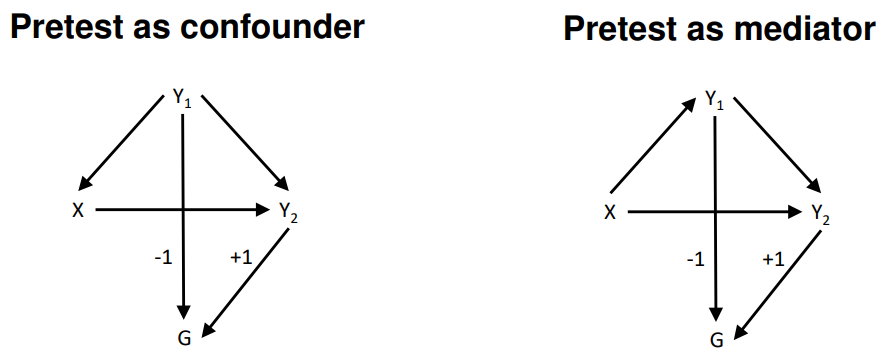
\includegraphics[width=0.55\textwidth]{changescoredag.png} \hfill 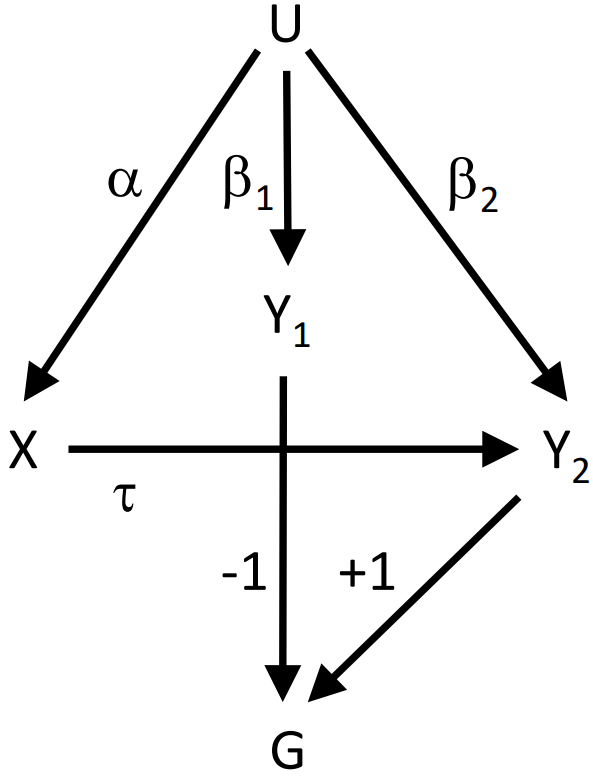
\includegraphics[width=0.19\textwidth]{unobservedconfounder_changescoredag.png}\\
\textbf{Lecture 6: Longitudinal DAG}\\
    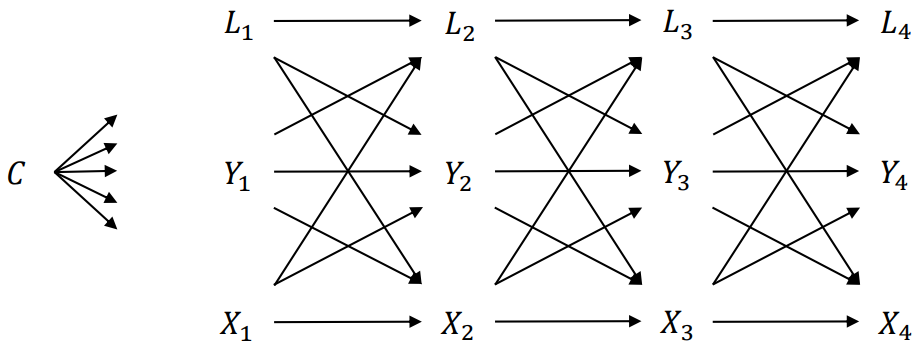
\includegraphics[width=0.5\textwidth]{jointtreatment.png}\\
\textbf{Lecture 7: RI-CLPM}\\
    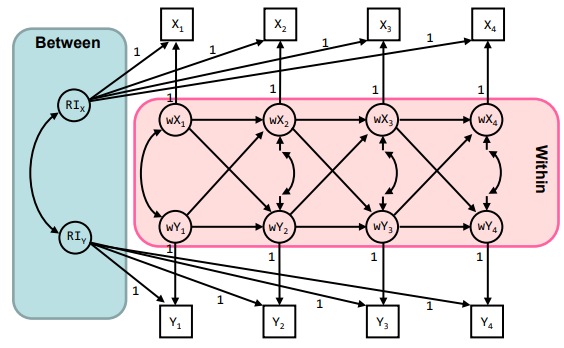
\includegraphics[width=0.57\textwidth]{riclpm.png}
\end{boxA}

%\begin{boxA}
%Longitudinal DAG:\\
%    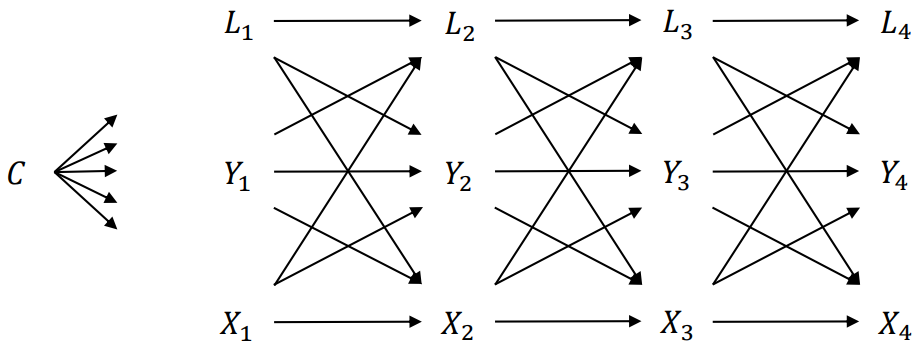
\includegraphics[width=\textwidth]{jointtreatment.png}
%\end{boxA}

INFOMDCSBS Cheat Sheet - Created by Tim Rentenaar

\end{multicols}

\end{document}
